\chapter{Introduction}

\section{Motivation}
Due to the rapid increase of mobile phones and other wireless communication 
devices, 
there is a need for efficient utilization of the available radio spectrum.
The Spectrum Policy Task Force, a group under the Federal Communications  
Commission (FCC) in the United States, published a report in 2002 saying 
\cite{repFCC}: 
\begin{quote}
``In many bands, spectrum access is a more significant problem than physical
scarcity of spectrum, in large part due to legacy command-and-control 
regulation that limits the ability of potential spectrum users to obtain such 
access.''
\end{quote}
If we scan the spectrum in metropolitan cities which are heavily used regions,
we find that some frequency bands are unoccupied most of the time\cite{staple04}. These 
are referred to as spectrum holes. A spectrum hole is a band of frequencies 
assigned to a primary user, but, at a particular time and specific geographic 
location, the band is not being utilized by that user\cite{kolodzy01}.

\begin{figure}
\centering
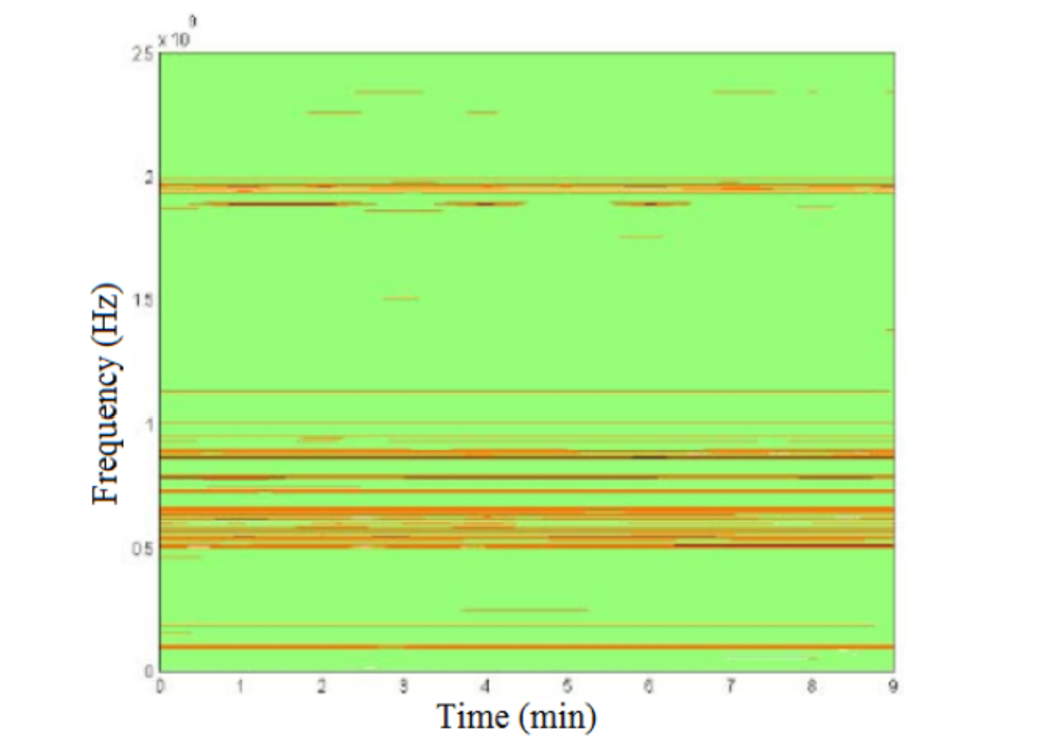
\includegraphics[width=0.7\textwidth]{../images/freqUsage}
\caption{Frequency usage of Spectrum Band}
\label{frequencyUsage}
\end{figure}


This problem of inefficient utilization of spectrum can be solved by allowing 
secondary users which are non licensed, to access these spectrum holes.
Cognitive radio which includes software defined radio, is a means to 
accomplish this by utilizing these spectrum holes intelligently and 
efficiently\cite{haykin05}\cite{mitola99}\cite{mitola00}. It uses one of the spectrum sensing techniques to 
identify the spectrum holes in the radio spectrum.


\section{Cognitive Radio}
A cognitive radio is an intelligent radio whose primary objective is efficient
utilization of the radio spectrum. It can be programmed and configured 
dynamically. It works on the principle of understanding-by-building to learn 
from the surrounding environment and adapt to changes in the RF stimuli by 
making corresponding changes in operating parameters. The transceiver is 
designed to find an unoccupied channel in the vicinity and utilize it for 
transmission. It enables coexistence of primary licensed users and secondary 
unlicensed users. Whenever a primary user wants to occupy the channel which is
currently in use by secondary users, it finds some other unoccupied channel in
the vicinity and secondary users migrate seamlessly to this new channel thus 
vacating the previously used channel for primary users.  

\section{Contribution of thesis}
An experimental setup is developed which demonstrates the presence of 
secondary users along with primary users in the existing GSM network and 
utilizing the already existing resources there by increasing the total 
mobiles in the network.
\begin{enumerate}
  \item A two frequency band cognitive system is developed where secondary 
  users migrate to frequency $f2$ if frequency $f1$ is occupied an viceverca.
  \item A two frequency system is extended to a four frequency system where 
  we demonstrate that primary users are occupying two bands out of these four
  and secondary users occupy one out of the other two free bands.
  \item We have used energy detection spectrum sensing technique and CUSUM
  peak detection technique to detect the presence of primary users. Band 
  occupied by secondary users is continuously monitored to check if primary 
  users are trying to occupy that band and as soon as the request from primary
  users is detected a new free band is found out in the vicinity and utilized 
  by secondary users for transmission there by vacating the band for primary 
  users . 
\end{enumerate}

\section{ORGANIZATION}
The rest of this document is organized as follows. Chapter 2 briefly describes
the GSM architecture and its Um interface. Chapter 3 gives a literature survey
on Universal Software Radio Peripheral (USRP N210) the hardware used in this 
project. Literature survey done on the GNU Radio software package and OpenBTS 
software is described in Chapter 4 and 5 respectively. Chapter 6 covers 
spectrum sensing techniques to detect the presence of primary users in the 
channel.  Chapter 7 covers an implementation of cognitive radio using GNU Radio
and OpenBTS. It describes the experimental setup for our project in the 
beginning followed by detailed description of what we have achieved in this 
project along with a flow chart of our work. The final chapter of this thesis 
is the conclusion of our project followed by future work. 
